\documentclass[wide,a4paper,titlepage,12pt] {article}
\usepackage{polski}
\usepackage[utf8]{inputenc}
\usepackage{listings}
\usepackage{slashbox}
\usepackage[table]{xcolor}
\usepackage{graphicx,pdflscape}
\usepackage{placeins}


\title{Grafika komputerowa}
\author{Tymon Tobolski (181037)}

% Title page layout (fold)
\makeatletter
\renewcommand{\maketitle}{
\begin{titlepage}
  \begin{center}
    \vspace*{3cm}
    \LARGE \@title \par
    \vspace{2cm}
    \textit{\small Autor:}\par
    \normalsize \@author\par \normalsize
    \vspace{3cm}
    \textit{\small Prowadzący:}\par
    Dr inż. Tomasz Kapłon \par
    \vspace{2cm}
    Wydział Elektroniki\\ III rok\\ Pn TP 08.15 - 11.00\par
    \vspace{4cm}
    \small 7 listopada 2011
  \end{center}
\end{titlepage}
}
\makeatother
  \lstset{
    language=c++,
    basicstyle=\ttfamily\scriptsize,
    numbers=left,
    numberstyle=\scriptsize,
    stepnumber=10,
    numbersep=9pt,
    showspaces=false,
    showstringspaces=false,
    showtabs=false,
    breaklines=true,
  }

\begin{document}
\maketitle
  \section{Cel laboratorium}
  \paragraph{}
  Celem laboratorium było zapoznanie sie z podstawowymi funkcjami biblioteki OpenGL oraz jej rozszerzenia GLUT.
  Poniższe zadania obejmuja rysowanie prostych kształtów w przestrzeni dwuwymiarowej.

  \section{Dywan sierpińskiego}
  \paragraph{}
  Program rysuje reprezentacje dywanu sierpińskiego
  o zadanym rozmiarze, stopniu przybliżenia oraz poziomie zniekształcenia.
  Wykorzystany algortym rekurencyjnie oblicza pozycje kolejnych kwadratów aż do
  osiągnięcia określonego poziomu. Na ostatnim poziomie rysowa są zniekształcone kwadraty, które układają się
  w przedstawiony poniżej wzór.

  \paragraph{}

  \lstinputlisting{dywan.cpp}

  \begin{figure}[htbp]
    \begin{center}
      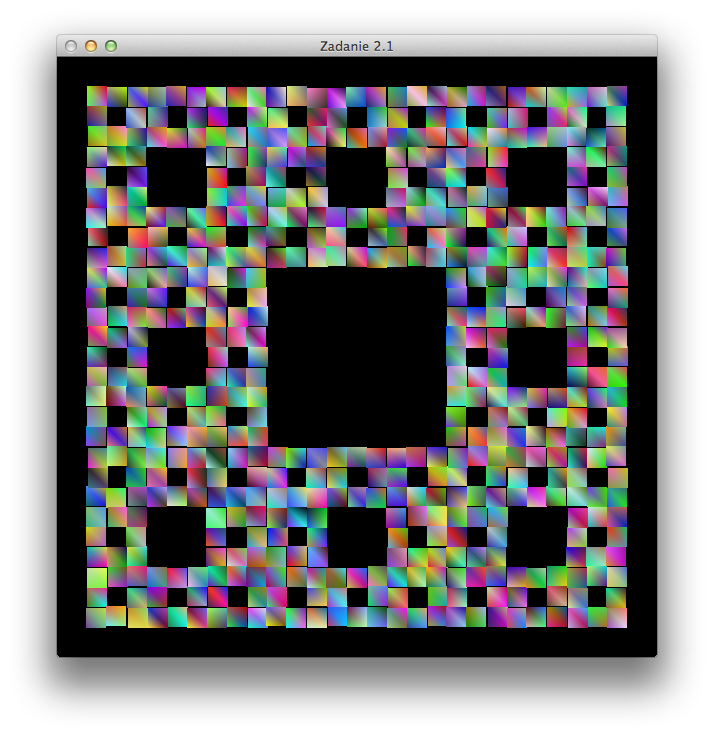
\includegraphics[scale=0.6]{dywan.png}
      \caption{Dywan sierpińskiego}
    \end{center}
  \end{figure}

  \newpage

  \section{Trójkąt sierpińskiego}
  \paragraph{}
  Pierwsza metoda rysowania trójkąta sierpińskiego polega na narysowaniu dużego trójkąta,
  a następnie "wycinaniu" mniejszego trójkąta ze środka poprzedniego. Czynność tę należy powtarzać,
  aż do otrzymania porządanego rezultatu.

  \paragraph{}
  Druga metoda rysowania trójkąta spierpińskiego polega na wybraniu losowego punktu
  w środku trójkąta, a następnie losowe przesuwanie sie w jednym z trzech kierunków,
  za każdym razem stawiając punkt.

  \paragraph{}

  \lstinputlisting{trojkat.cpp}

  \begin{figure}[htbp]
    \begin{center}
      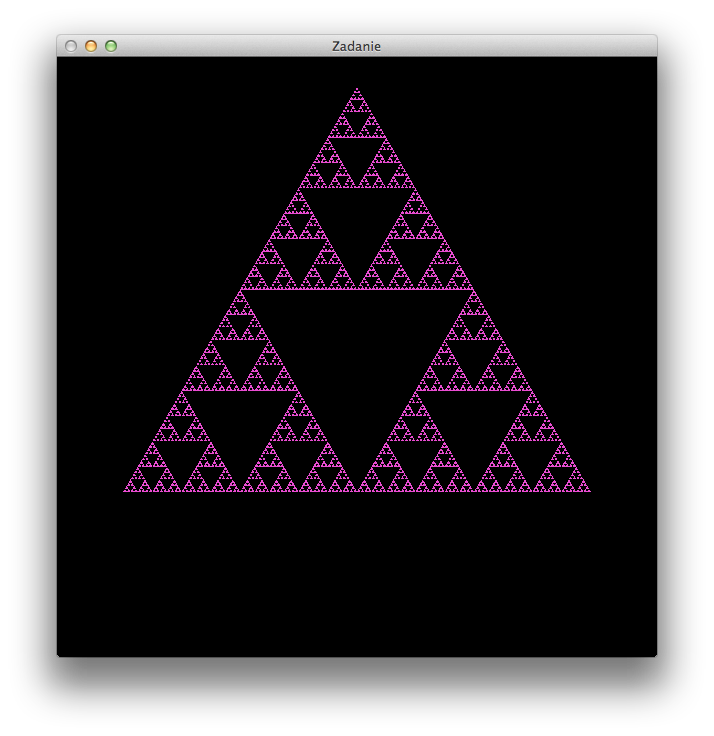
\includegraphics[scale=0.6]{trojkat.png}
      \caption{Trójkąt sierpińskiego}
    \end{center}
  \end{figure}


  \newpage


  \section{Labirynt}
  \paragraph{}

  Algortym generujący labirynt zaczyna się od wypełnienia powierzchni labiryntu siatką komnat o rozmiarach 1x1.
  Początek ustala się w dowolnym punkcie przy krawędzi labirytnu.
  Z każdym krokiem losowo wybierana jest sąsiadująca komnata, która posiada wszystkie ściany,
  ściana między wybraną komnata a obecna zostaje usunięta a algorytm zaczyna ponownie tę samą operacje
  od nowo otwartej komnaty. W przypadku braku sąsiadującej komnaty, która miała by wszystkie ściany program cofa się o jedno pole i ponawia poszukiwania.
  Algorytm kończy się kiedy wszystkie komnaty zostaną odwiedzone.

  \paragraph{}

  \lstinputlisting{maze.cpp}

  \begin{figure}[htbp]
    \begin{center}
      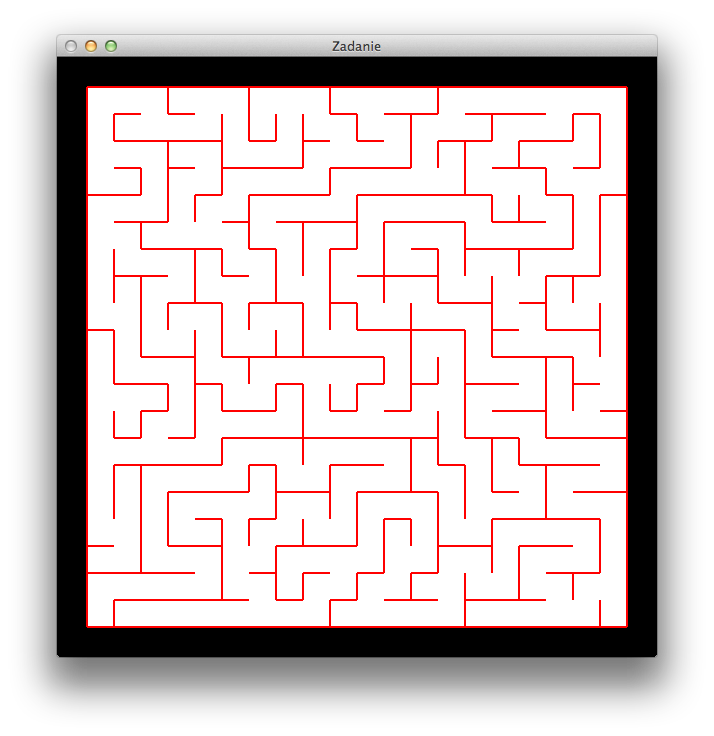
\includegraphics[scale=0.6]{maze.png}
      \caption{Labirynt}
    \end{center}
  \end{figure}

  \newpage

  \section{Fraktal plazmowy}
  \paragraph{}
  Program pozwala na rysowanie monochromatycznych jak i kolorowych fraktali plazmowych.
  Jedyną trudnością przy implementacji opisanego w dokumentacji algorytmu było dobranie
  odpowiednich funckji W(x) i Wc(x).

  \paragraph{}

  \lstinputlisting{fraktal.cpp}

  \begin{figure}[htbp]
    \begin{center}
      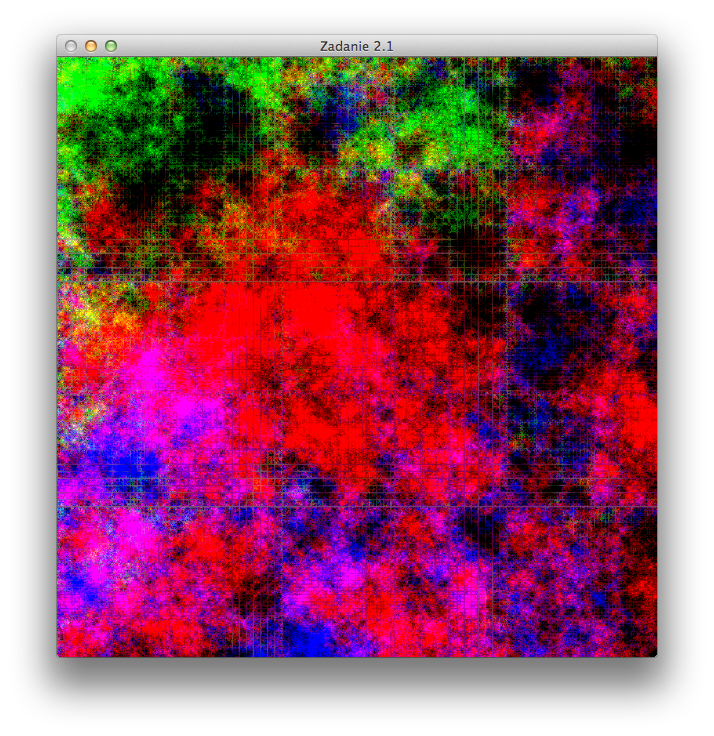
\includegraphics[scale=0.6]{fraktal.png}
      \caption{Fraktal plazmowy}
    \end{center}
  \end{figure}

  \newpage

  \section{Funkcje pomocnicze}
  \paragraph{}
  Poniżej znajdują się funkcje pomocnicze wykorzystywane w powyższych programach.
  \paragraph{}
  \lstinputlisting{misc.cpp}


\end{document}